% Study v3 paper draft. Compile with XeLaTeX (Arabic examples need fontspec):
%   latexmk -xelatex main.tex
% Requires acl.sty and acl_natbib.bst from https://github.com/acl-org/acl-style-files
% Everything marked \pending{...} depends on GPU runs or human annotation that have
% NOT been carried out yet; no number inside \pending is a result.
\documentclass[11pt]{article}
\usepackage[review]{acl}
\usepackage{fontspec}
\usepackage{booktabs}
\usepackage{graphicx}
\usepackage{xcolor}
\usepackage{microtype}
\newfontfamily\arabicfont[Script=Arabic]{Amiri}
\newcommand{\ar}[1]{{\arabicfont\RL{#1}}}
\providecommand{\RL}[1]{\beginR #1\endR}
\newcommand{\pending}[1]{\textcolor{red}{[PENDING: #1]}}
\newcommand{\unk}{\texttt{[UNK]}}

\title{One Character Erases a Word: Orthographic Noise, Tokenizers and\\Negation in Arabic Sentiment Models}

\author{Anonymous submission}

\begin{document}
\maketitle

\begin{abstract}
Arabic social media text routinely contains typographic elongation (tatweel), emphatic
letter repetition and inconsistent hamza and ta marbuta spelling. We audit how such
variation reaches five fine-tuned encoders and a zero-shot LLM on two tweet sentiment
datasets (ArSarcasm-v2 and ArSAS). A tokenizer-level audit of about 40,000 controlled
edits shows a sharp split. In all four Arabic WordPiece models we test, a single
tatweel turns the edited word into \unk{} in 100\% of cases, including every edited
negation cue. Multilingual byte-level tokenizers never produce an unknown token but
split the same word into 1.7--2.9 times as many pieces. Natural tatweel occurs in
3.2--4.6\% of tweets in both corpora. \pending{prediction flip rates per model and
condition, the cue-versus-non-cue contrast, and the effect of normalization defenses}.
We release perturbation code, leakage-safe splits and a preregistered analysis plan.
\end{abstract}

\section{Introduction}

Arabic sentiment classifiers are usually evaluated on the tweets their training data
came from, so their behaviour under ordinary orthographic variation is rarely measured
directly. Such variation is common. Writers stretch words with the tatweel character
(\ar{حلـــو}), repeat letters for emphasis (\ar{حلووو}, \ar{كثيييير}), and drop hamza
or write final \ar{ة} as \ar{ه}. In the two corpora we study, 3.2--4.6\% of tweets
contain at least one tatweel and 2.8--4.0\% repeat a letter three or more times
(Table~\ref{tab:natural}).

Earlier attempts to measure this robustness, including our own pilot, edited a single
word with a single model. They found effects too small to separate from zero. We argue
that such null results say more about the design than about the models. We therefore
ask four questions:
\begin{itemize}
\item[\textbf{RQ1}] How much do realistic orthographic edits change the predictions of
Arabic, multilingual and LLM-based sentiment models?
\item[\textbf{RQ2}] Do tokenizer effects explain the differences between models?
\item[\textbf{RQ3}] Is editing a negation cue more damaging than editing another word
in the same tweet?
\item[\textbf{RQ4}] Does inference-time normalization recover clean behaviour?
\end{itemize}

Our contributions are:
\begin{enumerate}
\item A deterministic perturbation suite with four families (tatweel, elongation,
spelling folding, and keyboard typos as a meaning-damaging control). Each family is
applied at two densities and with an explicit choice of whether the negation cue
itself is edited.
\item A tokenizer audit across six models and two datasets. It shows that tatweel
deletes a word for Arabic WordPiece vocabularies and that the effect replicates exactly
across corpora (\S\ref{sec:tokenizer}).
\item \pending{a multi-seed robustness analysis with paired cluster-bootstrap
intervals, a negation stress test and a defense ablation}.
\item Independent human validation of meaning preservation
\pending{$\kappa$ / AC1 from two expert annotators}, together with all code,
leakage-safe splits and a preregistration written before any prediction was observed.
\end{enumerate}

\section{Related work}

\paragraph{Noise robustness.} Synthetic and natural character noise both degrade
neural models \citep{belinkov2018synthetic}. Character-level defenses have been
proposed against misspellings \citep{pruthi-etal-2019-combating}, and behavioural test
suites probe such invariances directly \citep{ribeiro-etal-2020-beyond}. Our edits are
specific to Arabic script. We also separate presumed meaning-preserving edits from a
damaging control and validate the difference with human judgments.

\paragraph{Arabic pretrained models.} MARBERT \citep{abdul-mageed-etal-2021-arbert},
AraBERT \citep{antoun-etal-2020-arabert} and CAMeLBERT \citep{inoue-etal-2021-interplay}
use WordPiece vocabularies built from Arabic text. XLM-R \citep{conneau-etal-2020-unsupervised}
and Qwen2.5 \citep{qwen2.5} use multilingual subword vocabularies that cannot produce
unknown tokens. Recommended preprocessing for some Arabic models removes tatweel, but
nothing in the model interface enforces this.

\paragraph{Negation.} Benchmarks under-represent negation, and models often ignore it
\citep{hossain-etal-2020-analysis}. We do not parse negation scope. Instead, we compare
editing the cue itself with editing another word in the same tweet.

\section{Study design}
\label{sec:design}

The full analysis plan was preregistered before any model prediction on the new
perturbations was observed. The tokenizer audit in \S\ref{sec:tokenizer} was run
before the preregistration and is disclosed there as such.

\paragraph{Data.} ArSarcasm-v2 \citep{abu-farha-etal-2021-overview} is used with a
leakage-safe split that quarantines training tweets whose text occurs in the official
test set (10,037 train / 2,509 validation). ArSAS \citep{elmadany2018arsas} is
processed as follows:
\begin{itemize}
\item Mixed-sentiment tweets are removed.
\item Repeated tweet IDs and identical texts are merged into groups, and groups with
conflicting labels are excluded.
\item The remaining groups receive a stratified group split: 13,738 / 1,966 / 3,923.
\end{itemize}
We rejected ASTD \citep{nabil-etal-2015-astd} as the second dataset because 2,473
ArSarcasm-v2 training tweets (20\%) also occur in it. ArSAS shares a single
(excluded) tweet with ArSarcasm-v2. Development uses the validation partitions, and
both test partitions are evaluated once after the study is frozen.

\paragraph{Perturbations.} Each edit is chosen deterministically by hashing the tweet
ID and condition. URLs, mentions, hashtags and tokens attached to Latin characters are
never edited. The four families are:
\begin{itemize}
\item \emph{tatweel}: one \ar{ـ} inserted after the last joining letter of the word;
\item \emph{elongation}: the last internal long vowel (else the final letter) repeated
2 or 4 extra times;
\item \emph{folding}: \ar{أ}/\ar{إ}/\ar{آ}$\to$\ar{ا}, final \ar{ة}$\to$\ar{ه} and
final \ar{ى}$\to$\ar{ي};
\item \emph{typo}: one interior letter replaced by its neighbour on the Arabic
keyboard (the meaning-damaging control).
\end{itemize}
\emph{Single} conditions edit one word; \emph{dense} conditions edit
$\lceil 0.3\,\cdot\,$words$\rceil$. Single edits are nested within dense edits, and both
elongation levels edit the same character. \emph{Non-cue} conditions never touch an
unambiguous negation cue (\ar{لا}, \ar{لم}, \ar{لن}, \ar{ليس}, \ar{مش}, \ar{مو}, \ldots;
\ar{ما} is excluded as too ambiguous). \emph{Cue} conditions edit exactly that cue.
Table~\ref{tab:conditions} lists the number of applicable tweets.

\paragraph{Models.} We fine-tune MARBERT, MARBERTv2, AraBERTv02-twitter, CAMeLBERT-DA
and XLM-R-base with one fixed recipe:
\begin{itemize}
\item learning rate $2{\times}10^{-5}$, batch size 16, at most 5 epochs;
\item checkpoint selected by validation Macro-F1;
\item three seeds per model and dataset.
\end{itemize}
Qwen2.5-7B-Instruct is used zero-shot, with a fixed instruction and softmax over the
first-token logits of the three label words. All model revisions are pinned.

\paragraph{Defenses.} We compare four inference-time preprocessors:
\begin{itemize}
\item RAW: no change;
\item STD: removes tatweel and collapses runs of three or more identical letters;
\item NO\_CONTEXT and NASN2: two conservative normalizers carried over from our pilot.
NASN2 additionally abstains from editing near negation cues.
\end{itemize}

\paragraph{Metrics.} The primary metric is the \emph{flip rate}: the share of tweets
whose predicted class differs between the clean and perturbed text. Secondary metrics
are clean and perturbed Macro-F1 on the same tweets. Intervals are 95\% percentile
intervals from 2,000 cluster-bootstrap resamples over duplicate-text groups, with
seed-averaged rates inside each resample. Contrasts (cue vs.\ non-cue, dense vs.\ single,
defense vs.\ RAW, model vs.\ XLM-R) are paired on identical tweets.

\begin{table}[t]
\centering\small
\begin{tabular}{lrr}
\toprule
Condition & ArSarcasm-v2 & ArSAS \\
\midrule
tatweel / single / non-cue & 2,478 & 1,951 \\
tatweel / dense / non-cue & 2,478 & 1,951 \\
tatweel / single / cue & 404 & 316 \\
elongation$\times$2 / single / non-cue & 2,477 & 1,951 \\
elongation$\times$4 / single / non-cue & 2,477 & 1,951 \\
elongation$\times$2 / dense / non-cue & 2,477 & 1,951 \\
elongation$\times$2 / single / cue & 404 & 316 \\
folding / single / non-cue & 1,965 & 1,659 \\
folding / dense / non-cue & 1,963 & 1,657 \\
typo / single / non-cue & 2,476 & 1,951 \\
typo / dense / non-cue & 2,461 & 1,945 \\
\bottomrule
\end{tabular}
\caption{Validation tweets to which each condition applies (of 2,509 and 1,966).}
\label{tab:conditions}
\end{table}

\section{What the tokenizer sees}
\label{sec:tokenizer}

\begin{figure*}[t]
\centering
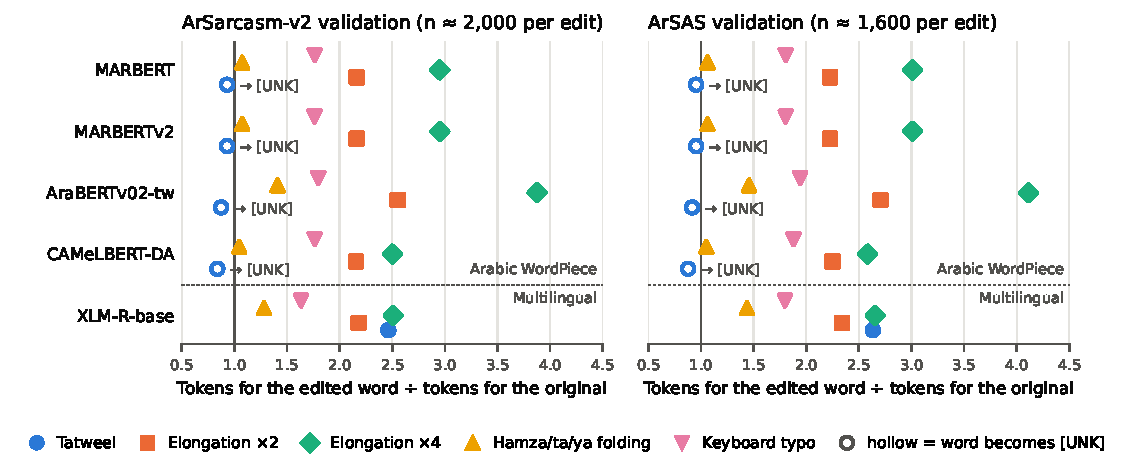
\includegraphics[width=\textwidth]{figures/tokenizer_edits.pdf}
\caption{Tokens produced for an edited word relative to its original, averaged over
single-word edits. A hollow marker means the edited word is mapped to \unk{} (rate 1.00
in every such cell). MARBERT and MARBERTv2 share a vocabulary, so their rows coincide.}
\label{fig:tokenizer}
\end{figure*}

Figure~\ref{fig:tokenizer} reports, for every model and edit family, how many tokens
the edited word receives relative to the original. Three patterns hold identically on
both datasets.

\paragraph{Tatweel deletes the word for Arabic WordPiece models.} In MARBERT,
MARBERTv2, AraBERTv02-twitter and CAMeLBERT-DA, every word containing an inserted
tatweel is tokenized as a single \unk{}. This happens in 100\% of single, dense and cue
edits on both datasets, including all 404 (ArSarcasm-v2) and 316 (ArSAS) edited
negation cues. None of the four vocabularies contains the tatweel character, so WordPiece
falls back to the unknown token for the whole word. A tweet with \ar{لـا} therefore
reaches these models with no negation at all.

\paragraph{Multilingual tokenizers fragment instead.} XLM-R and Qwen2.5 never produce
an unknown token. They split a word with one tatweel into 2.46 / 2.63 (XLM-R) and
1.92 / 2.02 (Qwen2.5) times as many pieces (ArSarcasm-v2 / ArSAS), and an edited
negation cue into 2.7--2.9 times as many.

\paragraph{Elongation fragments every model; spelling folding is partly absorbed.}
Four extra letters multiply the token count by 2.5--4.1, with AraBERTv02-twitter
highest (3.88 / 4.11). MARBERT's lower-casing strips hamza from alef, so 35.5\% / 30.9\%
of its single-word folding edits leave the token sequence unchanged. Every other
model sees nearly all folding edits.

These are statements about model inputs only. Whether an unknown token or a
fragmented word changes the prediction is the subject of \S\ref{sec:robustness}.

\section{Robustness of predictions}
\label{sec:robustness}

\pending{Table: flip rate and Macro-F1 drop with 95\% intervals per model, dataset and
condition (RAW). Test of H1 (dense $>$ single) and H2 (WordPiece $>$ XLM-R under dense
tatweel). Spearman correlation between per-cell \unk{} rate or fragmentation and flip
rate (RQ2).}

\paragraph{Natural noise.} \pending{On validation tweets that already contain tatweel
or letter runs, the flip rate and Macro-F1 difference between the tweet as written and
its STD-cleaned form.}

\section{Negation stress test}
Editing the negation cue itself is rare in the wild: five or fewer tweets per corpus
contain a naturally elongated or tatweel-marked cue (Table~\ref{tab:natural}). We
therefore treat the cue conditions as a controlled probe of how models encode negation,
not as an estimate of real-world risk. \pending{Paired cue minus non-cue flip-rate
differences (H3), restricted to tweets with a cue.}

\begin{table}[t]
\centering\small
\begin{tabular}{lrr}
\toprule
& ArSarcasm-v2 & ArSAS \\
\midrule
Tweets (train + validation) & 12,546 & 15,704 \\
with tatweel & 571 (4.6\%) & 502 (3.2\%) \\
with a letter repeated $\geq$3$\times$ & 498 (4.0\%) & 436 (2.8\%) \\
\quad of which a long vowel & 300 (2.4\%) & 294 (1.9\%) \\
with tatweel on a negation cue & 1 & 1 \\
with a repeated letter on a cue & 5 & 3 \\
\bottomrule
\end{tabular}
\caption{Naturally occurring noise. Test partitions were not read.}
\label{tab:natural}
\end{table}

\section{Do defenses help?}
\pending{STD vs.\ RAW (H4) and NASN2 vs.\ NO\_CONTEXT (H5). Our pilot found NASN2 and
NO\_CONTEXT to produce identical predictions on all 394 reviewed variants for MARBERT;
the preregistered rule claims an advantage for negation-aware abstention only if it
holds for at least three of five encoders.}

\section{Human validation}
\pending{Two independent native-speaker annotators, 330 items (30 per condition), with
the typo control as an attention check. Report Cohen's $\kappa$ and Gwet's AC1
\citep{gwet2008computing}, the share of items judged meaning- and
sentiment-preserving per family, and robustness restricted to human-confirmed items.}

\section{Conclusion}
\pending{Summary once predictions are in.} A practical recommendation already follows
from the tokenizer audit. Anyone deploying an Arabic WordPiece model on social media
text should strip tatweel before tokenization, because the model's own tokenizer will
otherwise silently delete the word.

\section*{Limitations}
\begin{itemize}
\item Edits are rule-based and placed one family at a time; real noise co-occurs.
\item The negation cue lexicon is finite and excludes \ar{ما}.
\item Validation partitions were used for checkpoint selection, which favours clean
accuracy (but not flip rate); the frozen test evaluation addresses this.
\item The LLM is evaluated with a single prompt.
\item Both datasets are tweets, so other genres may behave differently.
\end{itemize}

\section*{Ethics statement}
We use public research datasets under their licenses and release only tweet IDs,
hashes and labels, never tweet text. Two expert annotators
labelled the human-validation sample.

\bibliography{references}

\end{document}
